%%% LaTeX Template: Two column article
%%%
%%% Source: http://www.howtotex.com/
%%% Feel free to distribute this template, but please keep to referal to http://www.howtotex.com/ here.
%%% Date: February 2011

%%% Preamble
\documentclass[	DIV=calc,%
							paper=a4,%
							fontsize=12pt,%
							onecolumn]{scrartcl}	 					% KOMA-article class

\usepackage{lipsum}			% Package to create dummy text
\usepackage[brazil]{babel}	% English language/hyphenation
\usepackage[protrusion=true,expansion=true]{microtype}	% Better typography
\usepackage{amsmath,amsfonts,amsthm}					% Math packages
\usepackage[pdftex]{graphicx}							% Enable pdflatex
\usepackage[svgnames]{xcolor}			% Enabling colors by their 'svgnames'
\usepackage[hang, small,labelfont=bf,up,textfont=it,up]{caption}	% Custom captions under/above floats
\usepackage{epstopdf}						% Converts .eps to .pdf
\usepackage{subfig}							% Subfigures
\usepackage{booktabs}		% Nicer tables
\usepackage{float}
									
\usepackage{fix-cm}													% Custom fontsizes
\usepackage[utf8]{inputenc}
\usepackage[top=2.5cm, bottom=2.5cm, left=2.5cm, right=2.5cm]{geometry}
\usepackage[ddmmyyyy]{datetime}
\addto\captionsenglish{%
	\renewcommand\tablename{Tabela}
	\renewcommand\figurename{Figura}
} 
 

 
%%% Custom sectioning (sectsty package)
\usepackage{sectsty}													% Custom sectioning (see below)
\allsectionsfont{%															% Change font of al section commands
	\usefont{OT1}{phv}{b}{n}%										% bch-b-n: CharterBT-Bold font
	}

\sectionfont{%																% Change font of \section command
	\usefont{OT1}{phv}{b}{n}%										% bch-b-n: CharterBT-Bold font
	}



%%% Headers and footers
\usepackage{fancyhdr}												% Needed to define custom headers/footers
	\pagestyle{fancy}														% Enabling the custom headers/footers
\usepackage{lastpage}	

% Header (empty)
\lhead{}
\chead{}
\rhead{}
% Footer (you may change this to your own needs)

%% ====================================
%% ====================================
%% mude o rodape  do projeto
%% ====================================
%% ====================================

\lfoot{\footnotesize \texttt{Cabeamento estruturado} \textbullet ~Projeto}


\cfoot{}
\rfoot{\footnotesize Página \thepage\ de \pageref{LastPage}}	% "Page 1 of 2"
\renewcommand{\headrulewidth}{0.0pt}
\renewcommand{\footrulewidth}{0.4pt}



%%% Creating an initial of the very first character of the content
\usepackage{lettrine}
\newcommand{\initial}[1]{%
     \lettrine[lines=3,lhang=0.3,nindent=0em]{
     				\color{DarkBlue}
     				{\textsf{#1}}}{}}



%%% Title, author and date metadata
\usepackage{titling}															% For custom titles

\newcommand{\HorRule}{\color{DarkBlue}%			% Creating a horizontal rule
									  	\rule{\linewidth}{1pt}%
										}

\pretitle{\vspace{-30pt} \begin{flushleft} \HorRule 
				\fontsize{35}{35} \usefont{OT1}{phv}{b}{n} \color{DarkBlue} \selectfont 
				}

%% ====================================
%% ====================================
%% mude o titulo  do projeto
%% ====================================
%% ====================================

\title{Cabeamento Estruturado para Escritório de Pequenos Negócios}


% Title of your article goes here
%% ====================================



\posttitle{\par\end{flushleft}\vskip 0.5em}

\preauthor{\begin{flushleft}
					\large \lineskip 0.5em \usefont{OT1}{phv}{b}{sl} \color{DarkBlue}}
\author{Djeizon de Almeida Barros}  	% Author name goes here


\postauthor{\footnotesize \usefont{OT1}{phv}{m}{sl} \color{Black} 
					\\Universidade Tecnológica Federal do Paraná - Câmpus Cornélio Procópio 								% Institution of author
					\par\end{flushleft}\HorRule}

\date{}																				% No date




%%% Begin document
\begin{document}
\maketitle
\thispagestyle{fancy} 	
\thispagestyle{empty}		% Enabling the custom headers/footers for the first page 
% The first character should be within \initial{}


%% ====================================
%% ====================================
%% mude o resumo  do projeto
%% ====================================
%% ====================================

\initial{E}\textbf{ste projeto de cabeamento estruturado visa implementar, do zero, uma rede cabeada em um escritório de negócios, sob as normas vigentes com visada às boas práticas de instalação e manutenção dos componentes passivos. Cada vez mais presentes no mercado, os escritórios \textit{small business} são estruturas simples que possuem falta de infraestrutura e muitos desses locais ainda não estão completamente adaptados para suportar novas velocidades entregues pelos serviços de fibra óptica, disponibilizado na entrada da edificação, porém subutilizada pelo pobre cabeamento de cobre já entrando em fase de obsoletamento. O projeto contemplará o levantamento de planta física, elaboração da planta lógica, equipamentos passivos a serem implementados conforme a necessidade, os custos envolvidos para a devida implementação. Trata-se de projeto-modelo fictício para uso em diversas aplicações. No cenário atual em que diversas redes são erroneamente implementadas norteadas por práticas comuns e duvidosas, faz-se necessário um guia prático, pois, a leitura de normas textuais tornam-se praticamente ignoradas por pequenos negócios, seja pela dificuldade técnica de seus textos, falta de mão de obra para sua correta interpretação ou falta de orçamento para o direcionamento correto de custos.}


%% ====================================
\begin{figure}
	\centering
	
\includegraphics{utfpr}
\end{figure}

\vspace{2cm}
\centerline{\textit{\textbf{\today}}}

\clearpage
    \renewcommand*\listfigurename{Lista de figuras}
\listoffigures

\renewcommand*\listtablename{Lista de tabelas}
\listoftables




\clearpage
\renewcommand{\contentsname}{Sumário}
\tableofcontents
\clearpage

%% ====================================
%% ====================================
%% Inicio do texto
%% ====================================
%% ====================================
\section{Introdução}

Um novo serviço de internet é contratado por uma pequena empresa. O provedor de serviços para internet leva até o ponto do cliente o acesso à uma nova tecnologia: uso de fibra óptica. O pessoal que realiza essa instalação não informa o cliente de que os "500 megas" contratados poderá ser subutilizado caso a rede interna esteja completamente na base 10/100, isto é, suportando velocidades teóricas de, no máximo, 100 Mbps. Depois de um certo tempo, o empresário verifica que sua velocidade não ultrapassa os 92 Mbps (devido ao \textit{overhead} do roteador) e associa a baixa velocidade a um problema com o serviço do provedor de internet. Este vai ser, daqui para frente, o caso típico de muitas pequenas empresas que estão sob cabeamento estruturado obsoleto, utilizando equipamentos também obsoletos, todos operando na base 10/100 (FastEthernet).
\bigskip

Este projeto tem como finalidade, estabelecer um modelo de norte para adequadamente prestar-se atenção nos detalhes de uma nova instalação de cabeamento estruturado que suporte a base 10/100/1000 (Gigabit) e possa beneficiar-se ainda mais do custo-benefício do par metálico, com fornecimento do serviço de fibra óptica. Há detalhes importantes: desde um pequeno conector e seu banhamento metálico de ouro, até os equipamentos utilizados com finalidade de produzir redundância e alta disponibilidade para a empresa, haja vista que um pequeno negócio sem estar efetivamente \textit{online}, é empresa fadada ao fracasso.
\bigskip

\subsection{Escopo do Projeto}
O escopo deste projeto é a projeção de todos os componentes passivos de um cabeamento estruturado que será equipado com 25 computadores de mesa, 01 servidor, 01 roteador, 01 \textit{switch} e 04 pontos de acesso sem fio. Também se prevê redundância no acesso à Internet, com a contratação de dois provedores de serviços de internet. Apesar de o escopo não ser equipamentos ativos, serão descritos mais adiante uma recomendação para equipamentos ativos.

\subsection{Benefícios}
Hoje em dia, muitas redes cabeadas estão com capacidade parar suportar apenas velocidades teóricas de até 100 Mbps. A maioria dos roteadores de escritórios e/ou domésticos são comercializados como roteadores que operam na base 10/100. Quando se opta por um serviço de fibra óptica, nem todo micro-empresário está atento à subutilização do serviço devido às condições de instalação do cabeamento atual, podendo ocasionar algumas frustrações, tais como: gargalos na velocidade, má conexão devido à conectores prensados manualmente com alicates, conectores velhos, cabos dobrados indevidamente em determinado segmento do cabeamento. Nem todos os departamentos de T.I. possuem profissionais qualificados o suficiente para dominar todos os detalhes envolvidos numa instalação de cabeamento estruturado moderna. O benefício de ater-se às boas práticas de implementação de cabeamento estruturado é o marco inicial para que se possa realizar uma implementação que dure muitos anos.

\subsection{Organizações Envolvidas}
Em se tratando de projeto fictício, não há organizações envolvidas. Para fins de orientação, a seguinte tabela demonstra um conjunto de organizações, empresas ou profissionais que poderão eventualmente participar no envolvimento da implementação de uma rede.\\

% =======================================
% TABELINHA DE PROFISSIONAIS E ÓRGÃOS
% =======================================

\begin{table}[h!]
	\centering
	\renewcommand{\arraystretch}{2.0}
\caption{Possíveis organizações e profissionais envolvidos}
\label{tab1}
	\begin{tabular}{|l|l|}
		\hline
		\multicolumn{1}{|c|}{\textbf{Profissional / Empresa}} &	 \multicolumn{1}{|c|}{\textbf{Serviço}}                                 		  \\ \hline		Provedor de Internet 1                                
		& Serviço de acesso à Internet                                              \\ \hline
	    Provedor de Internet 2                               
	    & Serviço de acesso à Internet para redundância            					\\ \hline
		Engenheiro Elétrico                                  
		& Instalações elétricas relacionadas e não relacionadas à rede          \\ \hline
		Analista de Compras 
        & Orçamentos e compras de equipamentos          \\ \hline
		Projetista da Rede                                   
		& Projeta, configura e coloca em operação a rede lógica    \\ \hline
		Instalador da Rede                                   
		& Profissional ou equipe que instala a rede física           \\ \hline
		Telecom Local                                        
		& Instala/remaneja os troncos telefônicos         \\ \hline
		Empresa de Telefonia                                    
		& Profissional para instalar PABX e cabos telefônicos    \\ \hline
		ANATEL                                  
		& Órgão credenciador para certificação de redes \\ \hline
	\end{tabular}
\end{table}



% =======================================
% FIM DA TABELA
% =======================================


\section{Requisitos}

\subsection{Velocidade real contratada e percebida}
Toda a instalação deverá perceber a velocidade real do provedor de serviços de Internet contratado, acima de 100 Mbps, isto é, os \textit{hosts} deverão suportar as transmissões na base 10/100/1000, sem gargalos, bem como futuras atualizações de velocidade, até 1 Gbps.

\subsection{Extinção de conectores manualmente prensados com alicate}
Talvez um dos sintomas mais simples de um nó da rede que está apresentando falhas, fatalmente é devido a um conector estar manualmente prensado na ponta do fio de rede. Para obter algo próximo de uma rede certificada, é necessário que apenas se utilize a ferramenta de inserção (\textit{punch-down}) e um cordão injetado, comumente chamado de \textit{patch cord}.

\subsection{Tolerância à falha - Redundância contra quedas no serviço}
O roteador principal do escritório deverá receber dois sinais de WAN em duas interfaces, e deverá priorizar a mais veloz como a principal WAN; ao passo que, havendo um eventual blecaute e falta do sinal, o segundo provedor de internet assume o fornecimento de acesso, sem que o usuário final perceba que ocorreu um problema. Esta prática passou a ser mais comum devido à demanda das pequenas empresas realizarem operações de transferências de dados remotas com diversos fornecedores e clientes.

\subsection{Cobre de alta qualidade}
Para garantir uma boa longevidade da estrutura de instalação, sendo instalação nova, é preferível somente o uso de cabos de rede Categoria 6 (CAT6), por 03 motivos: \\ \\
(a) Geralmente possuem bitola maior no cobre;\\
(b) Possuem um septo separador que isola cada par trançado. Este separador fornece resistência física ao cabo e diminui aumenta o fenômeno chamado de \textit{cancelamento}, que ocorre nas correntes eletromagnéticas. Mais sobre \textit{cancelamento} é explicado na última subseção.\\
(c) São um bom custo benefício para redes Gigabit.\\

Em se tratando de cobre de alta qualidade, também se pensa em conectores corretos da Categoria 6, pois o uso de conectores da Categoria 5e poderão causar problemas de incompatibilidade pelas características físicas entre estas categorias. Eis que o conector CAT6 tem um melhor banho metálico em seus terminais.

\subsection{Todos os equipamentos ativos e passivos na base 1000}
Um bom cabeamento poderá ser rendido à completa subutilização se a rede estiver interligada à dispositivos que operam somente na base 10/100. Proritariamente, a compra de equipamentos --- roteadores, \textit{switches} e \textit{access points} --- deverá observar as características de que tais operam na base 10/100/1000, suportando as velocidades Gigabit.

\subsection{WiFi - Padrão IEEE 802.11ac implementado}
Este protocolo permite velocidades médias de 600Mbps nos pontos de acesso, ou seja, na data atual, uma referência muito boa para os padrões de Wi-Fi. (INSERIR REFERÊNCIA) Não é o escopo do projeto de cabeamento, mas a referência ao ponto de acesso correto certamente resultará em um sistema sem fio altamente eficiente.


\section{Usuários e Aplicativos}
O projeto visa atender um pequeno escritório que reúne um grupo de 9 profissionais. Não obstante, também considera a presença de dispositivos de rede, tais como impressoras cabeadas, pontos de acesso sem fio; e, usuários visitantes. No caso de pessoas não pertencentes ao local de trabalho, deverá ser implementada uma VLAN para dispositivos sem fio dos eventuais visitantes. No que se refere a cabeamento, a rede projetada deverá conter 2 pontos por área de trabalho (ATR), outros dois pontos nas áreas de impressora, incluindo pontos extras. Como o modelo é para satisfazer a escritórios de até, no máximo, 10 pessoas trabalhando, não há projeto de expansibilidade de imediato, no entanto, a projeção de pontos satisfaz uma futura expansibilidade sem demais custos. Os equipamentos a serem comprados são 01 roteador que suporte duas conexões WAN, 01 \textit{switch} de 48 portas, 04 pontos de acesso sem fio e respectivo cabeamento de par (04 vias) trançado. Sobre os equipamentos ativos, haverá a recomendação das marcas. Porém, a rede lógica fica a critério do departamento de T.I., em forma, aqui, de recomendações.

\subsection{Usuários}

Nesta seção será descrita a tabela de todos os profissionais atuantes na edificação que farão o uso do cabeamento estruturado e a explicação da rotina do acesso à rede de cada um deles.

% =======================================
% TABELA DE FUNCIONÁRIOS
% =======================================

\begin{table}[h!]
	\centering
	\caption{Tabela de funcionários e uso de aplicativos}
	\label{tab2}
	\renewcommand{\arraystretch}{2.0}
	\begin{tabular}{|l|l|}
		\hline
		\multicolumn{1}{|c|}{\textbf{Usuário}} &	 \multicolumn{1}{|c|}{\textbf{Aplicativos mais utilizados}}                                 		  \\ \hline		Diretor                                
		& Windows e Microsoft Office                                              \\ \hline
		Recepcionista                               
		& Windows e Microsoft Outlook            					\\ \hline
		Analista de T.I.                                  
		& Windows Server, SQL Server, RouterOS (MikroTik) ou Cisco IOS          \\ \hline
		Adminstrador 1 a 4 
		& Windows e Microsoft Office         \\ \hline
		Contador 1 e 2                                  
		& Windows, Microsoft Office e programas fiscais    \\ \hline
	\end{tabular}
\end{table}

% =======================================
% FIM DA TABELA
% =======================================

O \textbf{diretor da empresa} utilizar-se-á do sistema operacional Windows 10 e da suíte de aplicativos Microsoft Office. Grande parte da função do diretor é comandar a sua empresa, realizando contatos, conferindo planilhas no Servidor de Arquivos e comunicando-se com demais funcionários. É posição estratégica de liderança. Deve compreender que o uso bem empregado da tecnologia alavanque seus negócios, portanto deverá valorizar especialmente o Analista de T.I., pois seu negócio, além de estar disponível na Internet, precisa deste profissional como que na função de um "coringa", sempre apto a socorrê-lo numa situação de indisponibilidade com algum serviço.
\\ \\
O(a) \textbf{recepcionista} faz uso intenso do Microsoft Outlook, agendando compromissos, verificando e-mails a serem repassados e atendendo a telefonemas. Calendário e agendamento de compromissos é a palavra chave aqui. Também é o(a) profissional que é o "cartão de visita" da empresa, por conta do primeiro e subsequentes atendimentos prestados aos clientes.
\\ \\
O \textbf{Analista de Tecnologia da Informação} é o profissional que se encarregará de tomar conta da infraestrutura de rede, do servidor físico, da sala de equipamentos (SEQ) --- com acesso restrito --- equipamentos ativos e passivos de rede. Também será responsável pela manutenção de software, sendo os mais importantes o Windows Server e seus serviços críticos como o servidor de arquivos (\textit{File Server}), o servidor de banco de dados, usado pela contabilidade, e o sistema operacional RouterOS (bastante similiar ao CISCO IOS, nos roteadores CISCO). Tais tarefas também incluem rotinas de backup e contato com fornecedores de equipamentos e serviços de T.I.
\\ \\
Serão 04 funcionários atrelados à administração da empresa, \textbf{administradores} com diversas tarefas administrativas: folha de pagamento, impostos, contas a pagar, custos, despesas, compras e atividades bancárias. Disponibilidade de estar \textit{online} é essencial para esses funcionários.
\\ \\
Parte crítica da empresa e importantes funções são a de \textbf{contador}, em número de 02 pessoas. Além do uso do sistema operacional Windows, intenso uso do Microsoft Office, mais especificamente o aplicativo Excel e de programas fiscais exigidos pela Receita Federal. Fazem uso intensivo do banco de dados SQL Server, registrando empenhos e demais atividades de contabilidade considerados operações muito críticas.



\subsection{Aplicativos}

Nesta seção será descrita a tabela de aplicativos e suas funções críticas no negócio. As aplicações críticas levam à frente um asterisco (*).



% =======================================
% TABELA DE APLICATIVOS
% =======================================

\begin{table}[h!]
	\centering
\caption{Tabela de Aplicativos}
\label{tab3}
	\renewcommand{\arraystretch}{2.0}
	\begin{tabular}{|l|l|}
		\hline
		\multicolumn{1}{|c|}{\textbf{Aplicativo/Sistema}} &	 \multicolumn{1}{|c|}{\textbf{Descrição  de aplicativo}}                                 		  \\ \hline
		Windows Server 2016*                               
		& Servidor: File Server*, SQL Server*.                                               \\ \hline
		Windows 10                             
		& Sistema operacional das estações           					\\ \hline
		SQL Server                                  
		& Serviço do Windows Server*         \\ \hline
		RouterOS
		& Sistema operacional do roteador*        \\ \hline
		Microsoft Office                                  
		& Suite com aplicativos de escritório   \\ \hline
	\end{tabular}
\end{table}


% =======================================
% FIM DA TABELA
% =======================================

Nas estações de trabalho, impera-se pelo uso do sistema operacional \textbf{Microsoft Windows 10} (versão atual de compilação número 1930) e \textbf{Microsoft Office Professional 2016}, com as respectivas aplicações incorporadas: \\ 

\begin{itemize}
	\item Microsoft Word 2016 
	\item Microsoft Excel 2016
	\item Microsoft PowerPoint 2016
	\item Microsoft Outlook 2016
	\item Microsoft Publisher 2016
	\item Microsoft Access 2016
\end{itemize}



Conforme recomendação, é bom que o roteador utilize um sistema operacional com linha de comando, a exemplo dos modelos \textit{Mikrotik} ou CISCO. Esses sistemas fornecem o serviço DHCP e DNS para todos os \textit{hosts}, além de receber o \textit{link} de dois provedores de internet e balancear esta carga, caso um dos \textit{links} torne-se indisponível. Mais sobre estes equipamentos na seção {Recomendações}.
\\

Windows Server 2016. O sistema instalado no servidor do \textit{rack}. Opera sem virtualização, mas com RAID em modo de espelhamento (RAID 1) para criar alta redundância de dados. Não fornece DHCP, nem DNS, para não atrapalhar os serviços providos pelo roteador. \textit{Active Directory }não será implementado visto que não se trata de um escritório com mais de 50 máquinas. Serviços de hospedagem e nomes de domínio serão fornecidos por empresas de \textit{cloud computing} terceirizadas. No entanto, \textbf{SQL Server} interno deverá ser utilizado para guardar as informações consideradas sigilosas e críticas da empresa.


\section{Estrutura predial existente}

Trata-se de escritório de 9 cômodos, considerando também como cômodo, a área de circulação que é a área de ingresso ao andar. Situa-se numa edificação de um 01 térreo e 01 andar. O escritório em si é o 1º andar. O telhado da edificação é de fácil acesso físico, visto que a edificação é construída com bom madeiramento e telhas cerâmicas. A parte elétrica bem isolada, sem emaranhados de fios, o que facilita a retirada de algumas telhas para a travessia de alguns eletrodutos que comportarão os cabos, interligando o \textit{switch} e cada setor especificado. \\

As restrições de instalação são quebras da alvenaria mínimas. Os cabos deverão sofrer curvaturas de no máximo 45 graus e de volta em posição retilínea, seja ela vertical ou horizontal. As saídas dos pontos de rede deverão apresentar sua respectiva tomada externa, que deverão ser posicionadas à 40 centímetros do piso. Canaletas deverão ser utilizadas para a acomodação e boa visibilidade das instalações.
\\

Temos a área total de 109,12 metros quadrados, fragmentada em:

\begin{itemize}
	\item Sala de Reunião: 12,56.
	\item Sanitário e Pequena área: 6,41.
	\item Sala da Direção: 17,65.
	\item Sala da Administração 1 e 2: 12,74 (cada).
	\item Sala da Administração 2: 12,74.
	\item Sala da Contabilidade: 9,95.
	\item Sala da Recepção: 11,28.
	\item Sala de T.I.: 3,34.
	\item SEQ: 5,77.
	\item Circulação: 16,48.
	
	
\end{itemize}


%inicio dos comandos para criar uma nova pagina A3 horizontal
\clearpage 
\KOMAoptions{paper=a3, paper=landscape, DIV=20}
\recalctypearea

%\subsection{Planta Física com Mobília}


\begin{figure}
	%	\centering
	\noindent\makebox[\textwidth][c]{
		\includegraphics[width=\textwidth]{planta_01}
	}
	\caption{Planta física com mobília - Formato A3}
	\label{fig1}
\end{figure}

%Retornar ao formato A4
\clearpage
\KOMAoptions{paper=a4, paper=portrait, DIV=15}
\recalctypearea
%-- reinicio em A4 


\section{Planta Lógica - Elementos estruturados}

\subsection{Visão do cabeamento}
A planta lógica é apresentada na Figura 2. Conforme determina a norma, é necessário observar algumas coisas neste projeto. Primeiro, a variedade de plantas excedem por muitas vezes a própria norma, sendo impossível de se ter um padrão seguindo à risca. Segundo porque a própria norma torna opcional determinadas feituras num projeto, tal como a identificação por código de cor, quando uma edificação não tem mais que um pavimento.
\\

Para a simplificação da planta lógica, foram divididos, do \textit{switch}, portas que compreendem as numerações A, B, C e D. Sendo estas, \textbf{A: Portas 1-10}; \textbf{B: Portas 11-20}; \textbf{C: Portas 21-30} e \textbf{D: Portas 31-40}. Oito portas restantes ficam como suplementares em eventuais problemas com as portas utilizadas. As letras também indicam os eletrodutos que correm pela laje e descem por canaletas, passagens e posteriormente seguindo para e calhas verticais. 
\\

Observe-se que é importante neste agrupamento, meios de assegurar a melhor organização possível. No que tange às áreas de trabalho, são recomendados, no mínimo, 2 pontos por ATR, sendo pontos opcionais permitidos. Denominadas de ATR, as áreas de trabalho são pequenos espaços de trabalho, de um funcionário ou de dispositivos utilizados por funcionários, como impressoras e outros equipamentos. Os pontos RJ45 devem ser etiquetados com iniciação PT. Não é o caso de termos mais do que 01 \textit{switch} operando nesta rede, então foi simplificado o etiquetamento das saídas, como PT, duto de origem e/o grupo de portas com numeração.
\\

A Sala de Equipamentos (SEQ) é o local em que residirá o \textit{rack} da rede, comportando um \textit{switch} de 48 portas, e demais equipamentos ativos. Todos os equipamentos ativos, suportando o padrão Gigabit. Dá-se a subida dos cabos pela laje, pelo cômodo SEQ, com todos os cabos distribuídos em 04 caminhos, até o ponto de descida, indicados pelos \textit{spots} verdes, na figura. Na descida, encaminhar-se-ão por eletrocalhas fechadas e canaletas, até os \textit{keystones}, evitando ao máximo, que se prense conectores às terminações dos cabos. 
\\

Na planta, é possível observar que temos indicações de número de cabos dentro da canaleta ou, da calha. Em certos pontos, temos por certo que recebemos em torno de 8 cabos; e, com a ligação sequencial dos PTs, a quantidade de cabos vai diminuindo. É por isso que temos certas indicações como "4 x UTP" e "2 x UTP" na sequência: pois está contando em 02, tendo-se 02 cabos já tem previsão de estarem devidamente instalados, de 04 possíveis, naquele segmento. Importante observar que o manuseio dos cabos UTP sejam o mais cuidadoso possível: nenhuma dobra abaixo de 90, para que o cabo não perca suas características físicas e mecânicas de transmissão --- uma única dobra incorreta pode comprometer aquele ponto na rede. 
\\

Observa-se também, os pontos estratégicos de instalação de \textit{Wi-Fi}, bem como as impressoras de rede (\textit{Wi-Fi} 01 a 04), sendo posicionados para uma cobertura razoável de sinal sem fio. O QG, a entrada das comunicações, é o armário da edificação que comporta as entradas dos troncos telefônicos e da fibra óptica. Não é parte do projeto a estrutura de cabeamento telefônico, porém, vale dizer que é neste armário que está posicionada a Central de PABX híbrida. Caso ocorra alguma atualização dos equipamentos de telefonia, a rede já está preparada para suportar uma demanda de VoIP. 


%inicio dos comandos para criar uma nova pagina A3 horizontal
\clearpage
\KOMAoptions{paper=a3, paper=landscape, DIV=20}
\recalctypearea
%\subsection{Planta Física Cabeada}

\begin{figure}
	%	\centering
	\noindent\makebox[\textwidth][c]{
		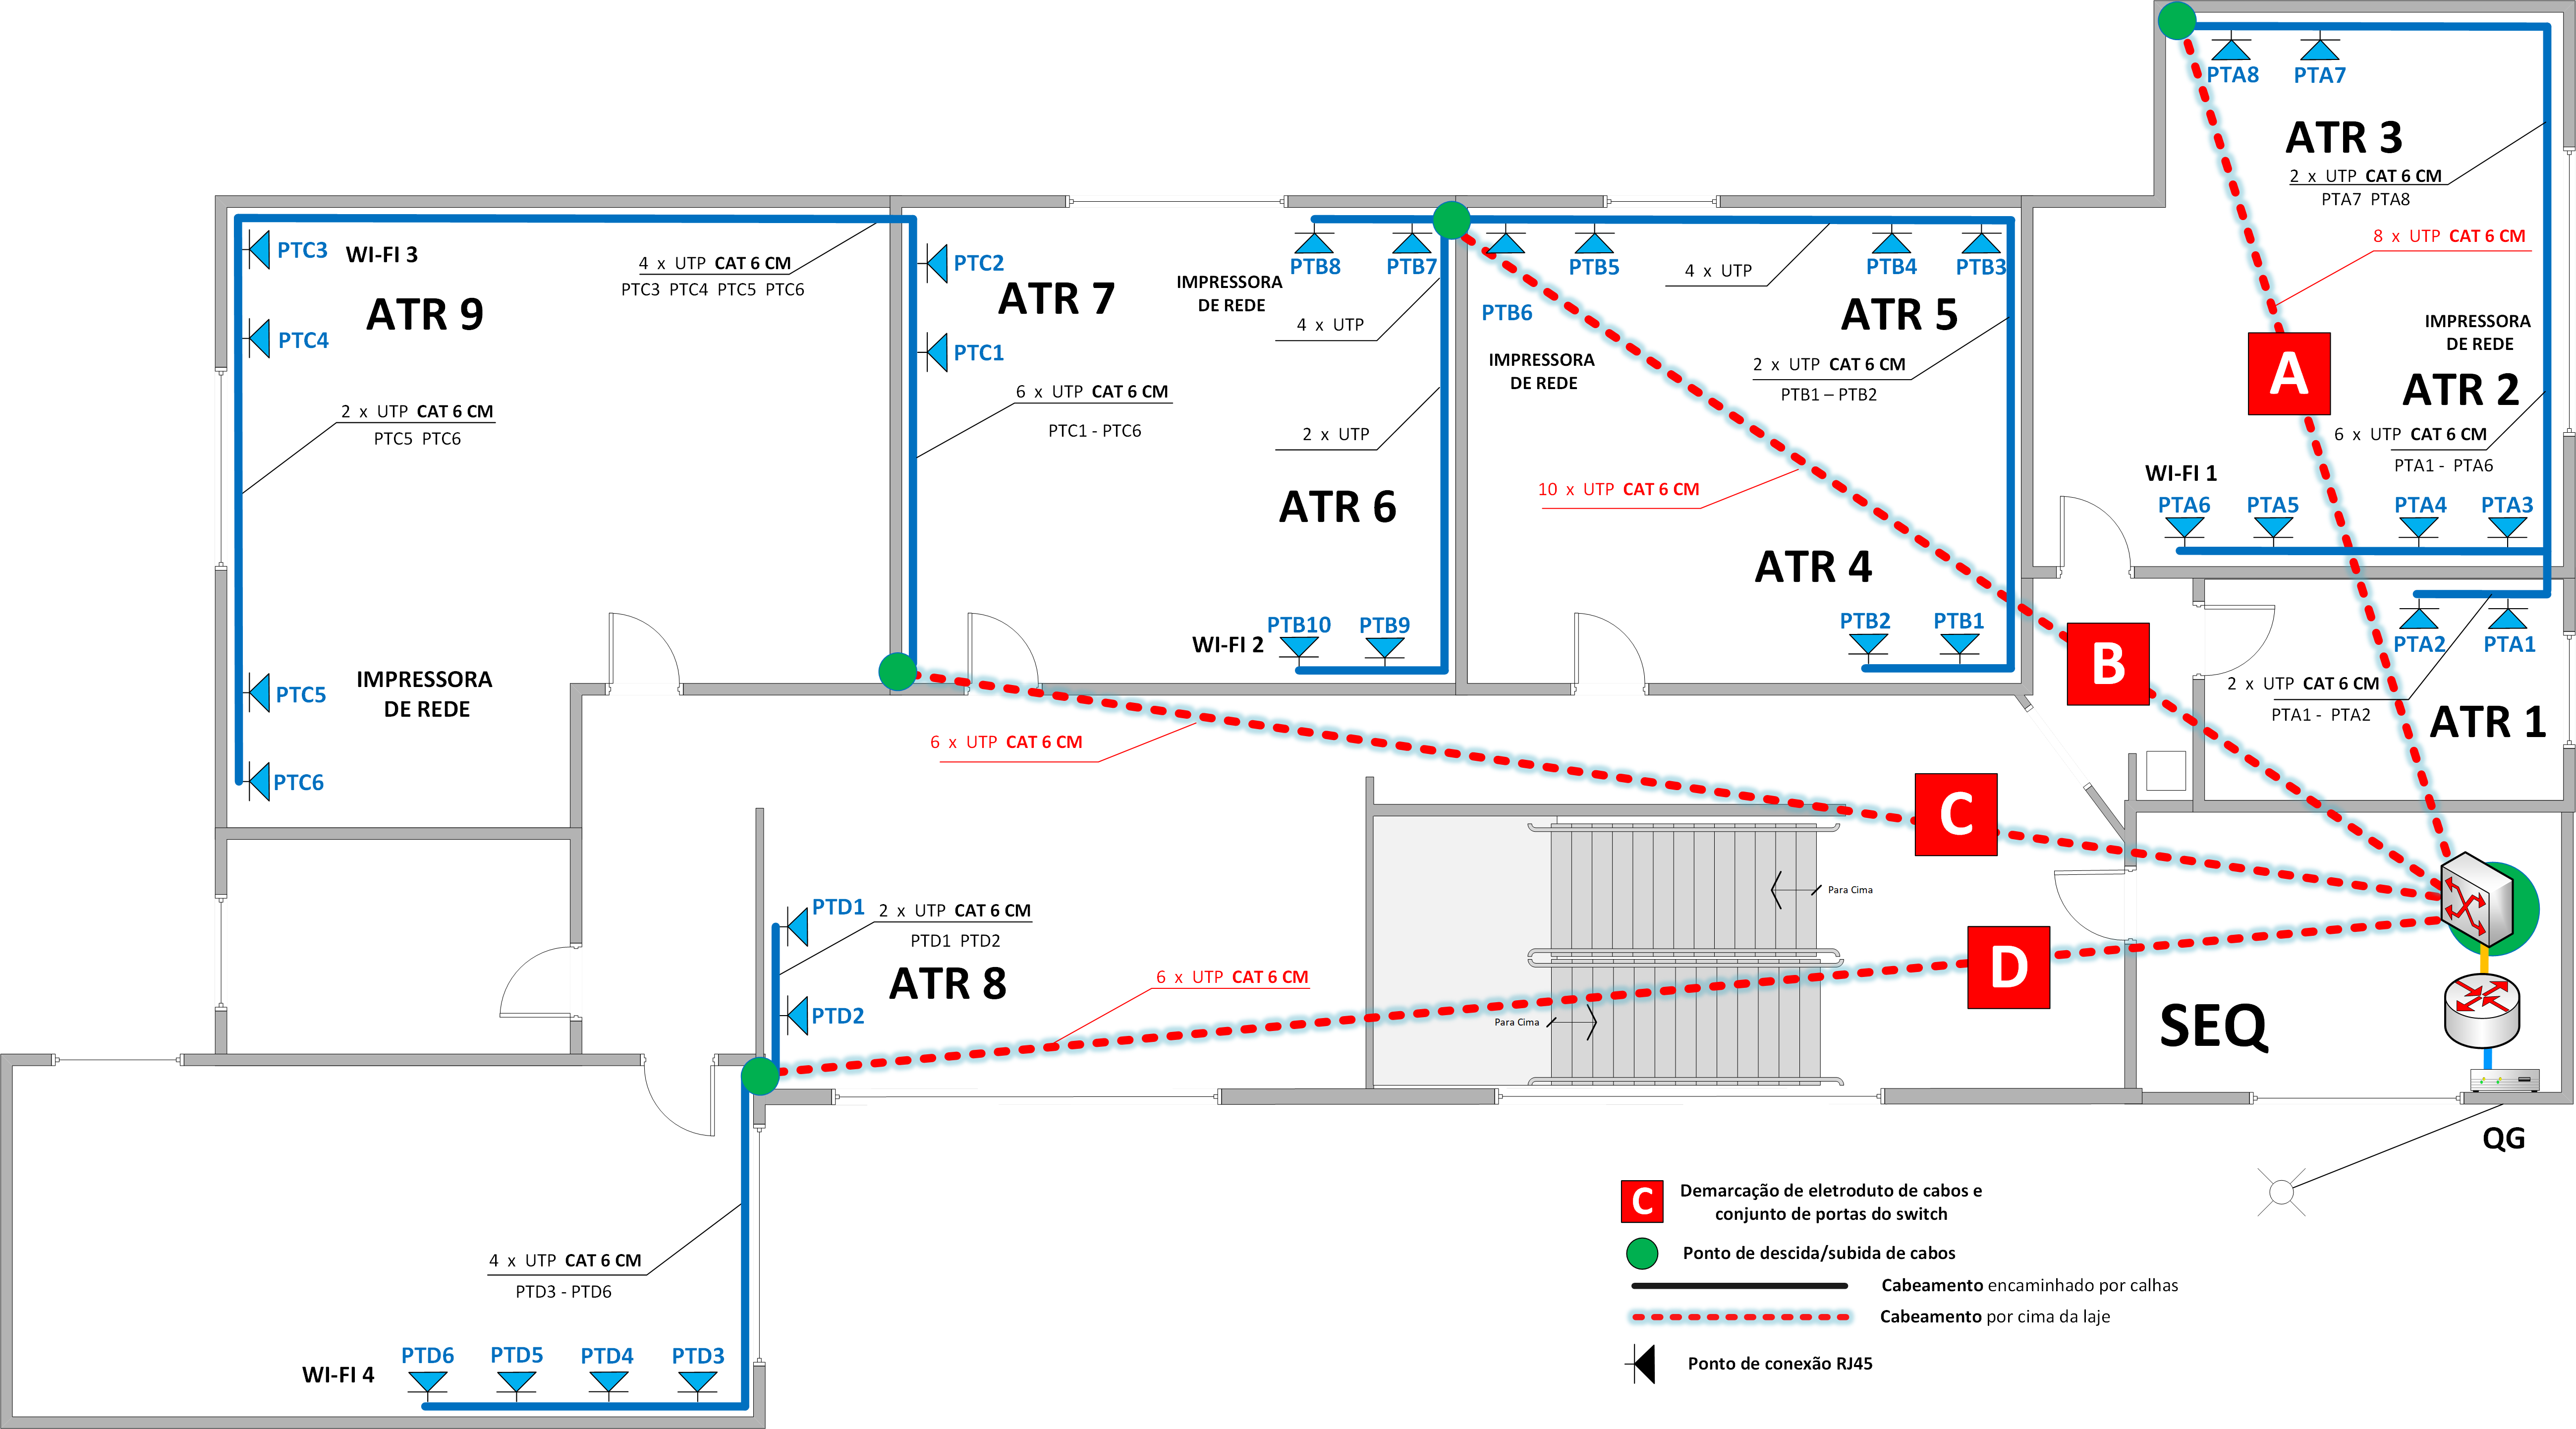
\includegraphics[width=\textwidth]{planta_02}
	}
	\caption{Planta lógica da visão do cabeamento - Formato A3}
	\label{fig1}
\end{figure}

%Retornar ao formato A4
\clearpage
\KOMAoptions{paper=a4, paper=portrait, DIV=15}
\recalctypearea
%-- reinicio em A4 











\subsection{Topologia}

A topologia de rede segue o modelo top-down e indica-se os elementos da maneira mais didática possível. Pode-se ver na imagem, que o projeto contempla duas entradas para a internet no roteador: WAN 1 e WAN 2. Diretamente ligado ao roteador, temos o \textit{switch} de 48 portas. Em uma das portas do \textit{switch}, o servidor de \textit{rack}. As ligações em vermelho, com marcações A, B, C e D, são os \textit{backbones} dos grupos de portas do \textit{switch}, mas que estão tomando diferentes caminhos, após a subida dos cabos.

% =======================================
% TABELA DE PORTAS DO SWITCH
% =======================================

\begin{table}[h!]
	\centering
\caption{Eletrodutos e portas de \textit{interface}.}
\label{tab4}
	\renewcommand{\arraystretch}{1.2}
	\begin{tabular}{|l|l|}
		\hline
		\multicolumn{1}{|c|}{\textbf{Letra do \textit{Backbone}}} &	 \multicolumn{1}{|c|}{\textbf{Portas}}                                 		  \\ \hline		A                                
		& 01, 02, 03, 04, 05, 06, 07, 08, 09*, 10*, 11*, 12*, 13*, 14*.                                             \\ \hline
		B                               
		& 15, 16, 17, 18, 19, 20, 21, 22, 23, 24, 25*, 26*, 27*, 28*.         					\\ \hline
		C                                  
		& 29, 30, 31, 32, 33, 34, 35*, 36*, 37*, 38*.          \\ \hline
		D 
		& 39, 40, 41, 42, 43, 44, 45*, 46*, 47*, 48*.         \\ \hline
		
	\end{tabular}
\end{table}


% =======================================
% FIM DA TABELA
% =======================================

Note-se que pelo cabeamento, as portas que recebem asterisco (*) são portas não utilizadas no \textit{switch}, mas com o cabeamento devidamente passado, para fins de redundância ou substituição de cabos. Conforme a população de cabos dentro do \textit{backbone}, tem-se mais cabos disponíveis para substituição.
\\

Conforme já demonstrado, os \textit{backbones} são cabeamentos majoritariamente horizontais, que terminam nos pontos de consolidação onde se começa a descida em cada cômodo. A única exceção que se faz é que esses \textit{backbones} totalizando 48 cabos, possuem uma parte na vertical, que sobem do \textit{rack} e vão até a laje, numa distância não mais que 2 metros.
\\

Dos pontos de consolidação, saem os cabos para todas as tomadas de conexão. No desenho, os dispositivos tais como computadores, impressoras, pontos de acesso sem fio e tomadas de conexão restantes são todos contabilizados como as saída de todos os cabos. Os retângulos em cinza indicam o cômodo em que determinado ponto de conexão ou dispositivo está instalado. Observe-se que determinado ponto de descida de \textit{backbone} pode alimentar outro cômodo, como é o exemplo do cômodo da Administração 1, no qual o cabeamento vertical, vai correr para o cômodo Administração 2.
\\

Os pontos de acesso sem fio são a exceção do cabeamento horizontal, pois, na verdade, esses dispositivos são instalados mais próximo à altura da porta (2,10 m) do que outros, dada a natureza de desejar-se boa cobertura de \textit{Wi-Fi}.
\\

Dentro dos tubos azuis, e das linhas vermelhas, é esperado uma determinada população de cabos (entre 10 e 14), enquanto que as linhas pretas não o cabeamento horizontal singular até a tomada e seu respectivo dispositivo. A linha pontilhada indica cabeamento vertical singular para o \textit{Wi-Fi}.



%inicio dos comandos para criar uma nova pagina A3 horizontal
\clearpage
\KOMAoptions{paper=a3, paper=landscape, DIV=20}
\recalctypearea
%\subsection{Topologia}

\begin{figure}
	%	\centering
	\noindent\makebox[\textwidth][c]{
		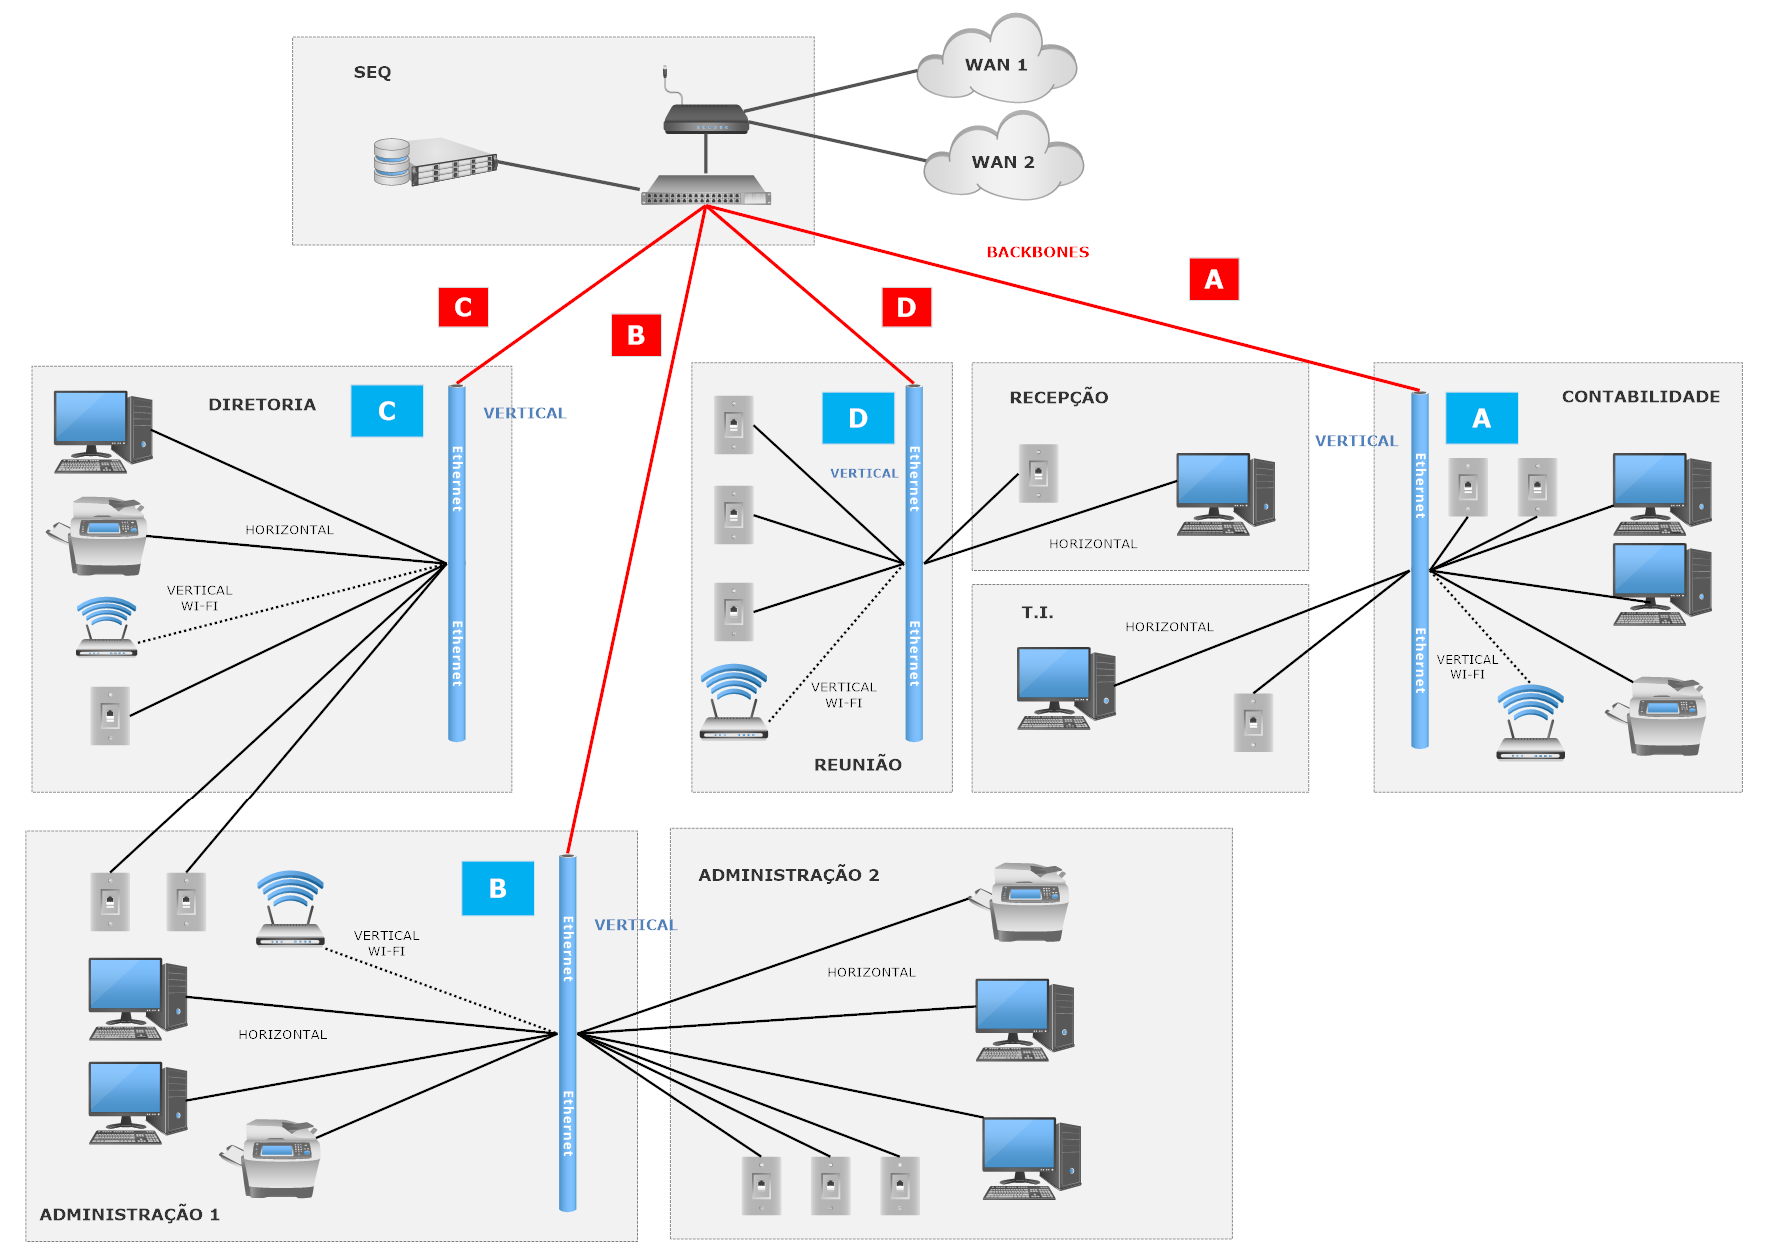
\includegraphics[width=\textwidth]{topologia}
	}
	\caption{Visão da topologia - Formato A3}
	\label{fig1}
\end{figure}

%Retornar ao formato A4
\clearpage
\KOMAoptions{paper=a4, paper=portrait, DIV=15}
\recalctypearea
%-- reinicio em A4 


\subsection{Encaminhamento}

Pela laje, serão instalados eletrodutos de PVC, de bitola de 2 polegadas. São vendidos em unidades de 3 metros. O sistema X2 de canaletas é versátil por ser adesivado, com alta aderência, e pode comportar até 12 cabos numa única canaleta (4 cabos por segmento, sendo 3 segmentos dentro da canaleta). Canaletas do sistema X são vendidas em unidades de 2 metros. Os acabamentos X2 trata-se de peças que se acoplam nas canaletas, tais como: cantos, curvas, e terminações onde não se é possível realizar manobras perigosas como a sobra massiva de cabos. Os acabamentos podem ser de diversas formas plásticas, mas aqui o ideal é que se pareçam com uma pequena caixa de inspeção nos cantos, para que os cabos possam ter ângulo suficiente de desvio, sem prejudicar as características físicas e mecânicas do CAT 6. Abaixo, uma tabela de quantidade de material de encaminhamento necessário para o cabeamento posterior ao \textit{backbone}.


% =======================================
% TABELA DE ENCAMINHAMENTO
% =======================================


\begin{table}[H]
\begin{center}
\caption{Encaminhamento previsto e peças relativas.}
\label{tab5}
	\renewcommand{\arraystretch}{1.2}
	\begin{tabular}{|c|c|c|c|}
		\hline
		\textbf{Tipo}       & \textbf{Fabricante} & \multicolumn{1}{l|}{\textbf{Metros}} & \multicolumn{1}{l|}{\textbf{Unidades}} \\ \hline
		Eletroduto PVC 4"         & Tigre               & 37,67                                   & 13                                     \\ \hline
		Canaleta X2 Adesivada         & Dutoplast             & 52,29                                  & 29                                     \\ \hline
		Acabamentos X2 & Dutoplast             & N/D                                  & 23                                     \\ \hline
			Dutos de passagem alvenaria & Tigre             & N/D                                  & 6                                     \\ \hline
	\end{tabular}
    	
\end{center}
\end{table}


\subsubsection{Calculo detalhado do encaminhamento}

% TABELA X2

\begin{table}[H]
\caption{Calculo detalhado --- canaletas X2.}
\label{tab6}
\begin{center}
	\renewcommand{\arraystretch}{1.2}
\begin{tabular}{|l|c|c|c|c|}
	\hline
	\multicolumn{5}{|c|}{\textbf{Canaletas X2 (em metros)}}                                                                                                 \\ \hline
	Trajeto da Canaleta & \multicolumn{1}{l|}{Trajeto A} & \multicolumn{1}{l|}{Trajeto B} & \multicolumn{1}{l|}{Trajeto C} & \multicolumn{1}{l|}{Trajeto D} \\ \hline
	Horizontal          & 9,90                           & 13,00                          & 10,80                          & 5,56                           \\ \hline
	Vertical            & 2,60                           & 5,20                           & 5,20                           & 5,20                           \\ \hline
	Subtotal (m)        & 12,50                          & 18,90                          & 16,40                          & 10,76                          \\ \hline
	\textbf{Total (m)}  & \multicolumn{4}{c|}{\textbf{52,29}}                                                                                               \\ \hline
\end{tabular}
\end{center}
\end{table}



% TABELA ELETRODUTOS
\begin{table}[H]
\caption{Calculo detalhado --- eletrodutos.}
\label{tab7}
\begin{center}
	\renewcommand{\arraystretch}{1.2}
\begin{tabular}{|l|c|c|c|c|}
	\hline
	\multicolumn{5}{|c|}{\textbf{Eletrodutos A/D}}                                                                            \\ \hline
	Trajeto do Eletroduto & \multicolumn{1}{l|}{A} & \multicolumn{1}{l|}{B} & \multicolumn{1}{l|}{C} & \multicolumn{1}{l|}{D} \\ \hline
	Horizontal            & 6,40                   & 8,46                  & 10,92                  & 11,89                   \\ \hline
	Vertical              & ---                    & ---                    & ---                    & ---                    \\ \hline
	\textbf{Total (m)}    & \multicolumn{4}{c|}{\textbf{37,67}}                                                               \\ \hline
\end{tabular}
\end{center}
\end{table}

% =======================================
% FIM DA TABELA
% =======================================


\subsection{Memorial descritivo (Passivos)}

Relação de todos os equipamentos passivos que serão utilizados, seguidos das tabelas com o respectivo custo destes passivos, bem como o custo do encaminhamento. Opta-se veementemente pelo uso de um \textit{rack} fechado, pois o local não tem a segurança adequada de um \textit{datacenter}. O cabo a ser orçado é da empresa Furukawa, líder no ramo. A peça 23400174 consiste da segunda linha, porém, superior ao cabo "comum" CAT 5e. A primeira linha, Gigalan, é de alto custo para o projeto, não compensando este investimento, mesmo em longo prazo. Os \textit{patch cords} são os elementos mais onerosos do projeto --- todos da marca Furukawa --- mas o sucesso da implementação depende de \textit{patch cords} de qualidade. A pequena variação de marca observa-se somente pelo conjunto de caixas de sobrepor e \textit{keystones}, mais econômicos, mas de qualidade, das marcas, respectivamente Central Network e AMP.

% =======================================
% TABELA DE PASSIVOS
% =======================================

\begin{table}[h!]
\caption{Equipamentos passivos}
\label{tab8}
\begin{center}
	\renewcommand{\arraystretch}{1.2}
	\begin{tabular}{|c|c|c|c|}
		\hline
		\textbf{Equipamento Passivo}      & \textbf{Fabricante} & \multicolumn{1}{l|}{\textbf{Quantidade}} \\ \hline
		Rack 44 U Fechado                 & Lextron             & 1                                \\ \hline
		Patch Panel 24 Portas CAT 6 GigaLan 35030162     & Furukawa          & 2                                \\ \hline
		Organizador 1 U 80 cm            & Lextron             & 2                               \\ \hline
		Cabo UTP CAT 6 Part 23400174 305 m                  & Furukawa            & 3        \\ \hline
			Cabo UTP CAT 6 Part 23400174 70 m                  & Furukawa            & 1        \\ \hline
	
		Patch Cords CAT 6 - 1,5 m (Cinza) & Furukawa                 & 38                            \\ \hline
		Patch Cords CAT 6 - 2,5 m (Cinza) & Furukawa                 & 22                             \\ \hline
		Caixa de Sobrepor 1 Porta              & Central Network              & 40                             \\ \hline
		Keystone 375055-1
		 CAT 6                   & AMP              & 40                             \\ \hline
	\end{tabular}
\end{center}
\end{table}


% =======================================
% FIM DA TABELA
% =======================================

\subsubsection{Calculo detalhado do cabeamento e considerações sobre emendas}

Na tabela da próxima página, temos o cálculo detalhado do quanto de cabo é estimado para que se saia do \textit{patch panel} e chegue-se até o ponto da área de trabalho. Uma coisa que se deve evitar quando se lida com cabos de cobre é a emenda. A emenda só pode ocorrer quando a situação for extremamente urgente: um serviço indisponível pelo rompimento de um cabo; uma situação de manutenção provisória. Seja qual for o tipo de emenda, precisa ser executada com muita habilidade e precisão: com as ferramentas e conectores corretos. As emendas causam atenuações no sinal. A prática de soldar emendas com a combinação estanho/chumbo, causa um ponto de resistência de elétrons e deve ser "abominada" num projeto, até mesmo por projetos de elétrica. (CITAR REFERENCIA) 




\clearpage

\KOMAoptions{paper=a3, paper=landscape, fontsize=11pt, DIV=20}
\recalctypearea

{\centering
\begin{table}[h!]
	\caption{Descrição detalhada do cabeamento --- em metros.}
	\label{tab9}
\begin{tabular}{|c|c|c|c|c|c|c|c|c|}
	\hline

	\textbf{Porta}     & \textbf{Ponto}     & \multicolumn{1}{l|}{\textbf{Do Patch Panel ao Teto}} & \multicolumn{1}{l|}{\textbf{No Eletroduto}} & \multicolumn{1}{l|}{\textbf{Descida do teto}} & \multicolumn{1}{l|}{\textbf{Subida até o AP}} & \multicolumn{1}{l|}{\textbf{Caminho horizontal}} & \multicolumn{1}{l|}{\textbf{Sobra Salvaguarda}} & \multicolumn{1}{l|}{\textbf{Total do Cabo Cortado Ponto a Ponto}} \\ \hline
	01                 & PTA1               & 2                                                    & 6,4                                         & 2,6                                           & ---                                           & 6,63                                             & 0,35                                            & 17,98                                                             \\ \hline
	02                 & PTA2               & 2                                                    & 6,4                                         & 2,6                                           & ---                                           & 7,25                                             & 0,35                                            & 18,60                                                             \\ \hline
	03                 & PTA3               & 2                                                    & 6,4                                         & 2,6                                           & ---                                           & 6,62                                             & 0,35                                            & 17,97                                                             \\ \hline
	04                 & PTA4               & 2                                                    & 6,4                                         & 2,6                                           & ---                                           & 7,23                                             & 0,35                                            & 18,58                                                             \\ \hline
	05                 & PTA5               & 2                                                    & 6,4                                         & 2,6                                           & ---                                           & 8,24                                             & 0,35                                            & 19,59                                                             \\ \hline
	06                 & PTA6               & 2                                                    & 6,4                                         & 2,6                                           & 2                                             & 8,86                                             & 0,35                                            & 20,21                                                             \\ \hline
	07                 & PTA7               & 2                                                    & 6,4                                         & 2,6                                           & ---                                           & 0,25                                             & 0,35                                            & 11,60                                                             \\ \hline
	08                 & PTA8               & 2                                                    & 6,4                                         & 2,6                                           & ---                                           & 0,88                                             & 0,35                                            & 12,23                                                             \\ \hline
	09                 & PTA R1             & 2                                                    & 6,4                                         & 2,6                                           & ---                                           & 8,9                                              & 0,35                                            & 20,25                                                             \\ \hline
	10                 & PTA R2             & 2                                                    & 6,4                                         & 2,6                                           & ---                                           & 8,9                                              & 0,35                                            & 20,25                                                             \\ \hline
	11                 & PTA R3             & 2                                                    & 6,4                                         & 2,6                                           & ---                                           & 8,9                                              & 0,35                                            & 20,25                                                             \\ \hline
	12                 & PTA R4             & 2                                                    & 6,4                                         & 2,6                                           & ---                                           & 8,9                                              & 0,35                                            & 20,25                                                             \\ \hline
	13                 & PTA R5             & 2                                                    & 6,4                                         & 2,6                                           & ---                                           & 8,9                                              & 0,35                                            & 20,25                                                             \\ \hline
	14                 & PTA R6             & 2                                                    & 6,4                                         & 2,6                                           & ---                                           & 8,9                                              & 0,35                                            & 20,25                                                             \\ \hline
	15                 & PTB1               & 2                                                    & 8,46                                        & 2,6                                           & ---                                           & 8,92                                             & 0,35                                            & 22,23                                                             \\ \hline
	16                 & PTB2               & 2                                                    & 8,46                                        & 2,6                                           & ---                                           & 8,27                                             & 0,35                                            & 21,68                                                             \\ \hline
	17                 & PTB3               & 2                                                    & 8,46                                        & 2,6                                           & ---                                           & 3,58                                             & 0,35                                            & 16,99                                                             \\ \hline
	18                 & PTB4               & 2                                                    & 8,46                                        & 2,6                                           & ---                                           & 2,94                                             & 0,35                                            & 16,35                                                             \\ \hline
	19                 & PTB5               & 2                                                    & 8,46                                        & 2,6                                           & ---                                           & 0,97                                             & 0,35                                            & 14,38                                                             \\ \hline
	20                 & PTB6               & 2                                                    & 8,46                                        & 2,6                                           & ---                                           & 0,36                                             & 0,35                                            & 13,77                                                             \\ \hline
	21                 & PTB7               & 2                                                    & 8,46                                        & 2,6                                           & ---                                           & 0,14                                             & 0,35                                            & 13,55                                                             \\ \hline
	22                 & PTB8               & 2                                                    & 8,46                                        & 2,6                                           & ---                                           & 0,82                                             & 0,35                                            & 14,23                                                             \\ \hline
	23                 & PTB9               & 2                                                    & 8,46                                        & 2,6                                           & ---                                           & 3,49                                             & 0,35                                            & 16,90                                                             \\ \hline
	24                 & PTB10              & 2                                                    & 8,46                                        & 2,6                                           & 2                                             & 4,09                                             & 0,35                                            & 17,50                                                             \\ \hline
	25                 & PTB R1             & 2                                                    & 8,46                                        & 2,6                                           & ---                                           & 9                                                & 0,35                                            & 22,41                                                             \\ \hline
	26                 & PTB R2             & 2                                                    & 8,46                                        & 2,6                                           & ---                                           & 9                                                & 0,35                                            & 22,41                                                             \\ \hline
	27                 & PTB R3             & 2                                                    & 8,46                                        & 2,6                                           & ---                                           & 9                                                & 0,35                                            & 22,41                                                             \\ \hline
	28                 & PTB R4             & 2                                                    & 8,46                                        & 2,6                                           & ---                                           & 9                                                & 0,35                                            & 22,41                                                             \\ \hline
	29                 & PTC1               & 2                                                    & 10,92                                       & 2,6                                           & ---                                           & 2,77                                             & 0,35                                            & 18,64                                                             \\ \hline
	30                 & PTC2               & 2                                                    & 10,92                                       & 2,6                                           & ---                                           & 2,15                                             & 0,35                                            & 18,02                                                             \\ \hline
	31                 & PTC3               & 2                                                    & 10,92                                       & 2,6                                           & 2                                             & 7,98                                             & 0,35                                            & 23,85                                                             \\ \hline
	32                 & PTC4               & 2                                                    & 10,92                                       & 2,6                                           & ---                                           & 8,58                                             & 0,35                                            & 24,45                                                             \\ \hline
	33                 & PTC5               & 2                                                    & 10,92                                       & 2,6                                           & ---                                           & 11,04                                            & 0,35                                            & 26,91                                                             \\ \hline
	34                 & PTC6               & 2                                                    & 10,92                                       & 2,6                                           & ---                                           & 11,66                                            & 0,35                                            & 27,53                                                             \\ \hline
	35                 & PTC R1             & 2                                                    & 10,92                                       & 2,6                                           & ---                                           & 12                                               & 0,35                                            & 27,87                                                             \\ \hline
	36                 & PTC R2             & 2                                                    & 10,92                                       & 2,6                                           & ---                                           & 12                                               & 0,35                                            & 27,87                                                             \\ \hline
	37                 & PTC R3             & 2                                                    & 10,92                                       & 2,6                                           & ---                                           & 12                                               & 0,35                                            & 27,87                                                             \\ \hline
	38                 & PTC R4             & 2                                                    & 10,92                                       & 2,6                                           & ---                                           & 12                                               & 0,35                                            & 27,87                                                             \\ \hline
	39                 & PTD1               & 2                                                    & 11,87                                       & 2,6                                           & ---                                           & 1,05                                             & 0,35                                            & 17,87                                                             \\ \hline
	40                 & PTD2               & 2                                                    & 11,87                                       & 2,6                                           & ---                                           & 0,38                                             & 0,35                                            & 17,20                                                             \\ \hline
	41                 & PTD3               & 2                                                    & 11,87                                       & 2,6                                           & ---                                           & 2,62                                             & 0,35                                            & 19,44                                                             \\ \hline
	42                 & PTD4               & 2                                                    & 11,87                                       & 2,6                                           & ---                                           & 3,24                                             & 0,35                                            & 20,06                                                             \\ \hline
	43                 & PTD5               & 2                                                    & 11,87                                       & 2,6                                           & ---                                           & 3,88                                             & 0,35                                            & 20,70                                                             \\ \hline
	44                 & PTD6               & 2                                                    & 11,87                                       & 2,6                                           & 2                                             & 4,52                                             & 0,35                                            & 21,34                                                             \\ \hline
	45                 & PTD R1             & 2                                                    & 11,87                                       & 2,6                                           & ---                                           & 4,6                                              & 0,35                                            & 21,42                                                             \\ \hline
	46                 & PTD R2             & 2                                                    & 11,87                                       & 2,6                                           & ---                                           & 4,6                                              & 0,35                                            & 21,42                                                             \\ \hline
	47                 & PTD R3             & 2                                                    & 11,87                                       & 2,6                                           & ---                                           & 4,6                                              & 0,35                                            & 21,42                                                             \\ \hline
	48                 & PTD R4             & 2                                                    & 11,87                                       & 2,6                                           & ---                                           & 4,6                                              & 0,35                                            & 21,42                                                             \\ \hline
	\multicolumn{2}{|c|}{\textbf{Subtotal}} & 96                                                   & 435,94                                      & 124,8                                         & 8                                             & 295,21                                           & 16,8                                            & 976,75                                                            \\ \hline
	\multicolumn{2}{|c|}{\textbf{Total}}    & \multicolumn{7}{c|}{976,75}                                                                                                                                                                                                                                                                                                                                                 \\ \hline
\end{tabular}
\end{table}
}

%Retornar ao formato A4
\clearpage
\KOMAoptions{paper=a4, paper=portrait, DIV=15}
\recalctypearea
%-- reinicio em A4 

\subsection{Identificação dos cabos}

Os cabos serão identificados pela seguinte nomenclatura:
\\

\textbf{PT} = Ponto da \textbf{Área de Trabalho.}
\\

\textbf{A} = Letra indicadora do \textbf{Eletroduto de Cabos} / Grupo de Portas.
\\

\textbf{1} = Número do cabo.
\\

\textbf{R} = Letra indicadora de \textbf{Cabo Reserva}.
\\

\textbf{1} = Número após o R indica o cabo reserva em questão.
\\

Os cabos reservas passam pelos eletrodutos, porém eles não descem pelas canaletas de distribuição. A sobra destes condutores ficam armazenadas numa caixa protegida em cima da própria laje, sem adentrar o duto de passagem vertical, especialmente no começo dos pontos de descida dos cabos. Porém, eles ficam suspensos até o \textit{rack}, na origem do sinal: assim caso algum cabo venha a estar danificado na certificação, a manobra para substituir aquele por outro cabo já passado resumir-se-á apenas pela prensagem deste no \textit{patch panel} e na outra extremidade, sim, a recuperação da sobra, pela laje.
\\

Os \textit{patch cords} são identificados com etiquetadoras, bem como os cabos que saem com uma pequena sobra salvaguarda das canaletas.

\section{Implantação}

\textbf{\begin{center}
		FAZER AQUI URGENTE
\end{center}}

Estabeleça um cronograma de implantação:
Remoção de equipamentos existentes (destino para descarte), instalação dos condutores, instalação dos cabos, 
identificação dos cabos, montagem dos racks, certificação, etc... Crie atividades e estabeleça o tempo de execução. Se for um projeto real, indique também quais os responsáveis pela execução do projeto e de cada uma das etapas.

Defina marcas (e padrões) e fornecedores se for o caso. Atenção a contratados e subcontratados para a realização das atividades. Estabeleça a responsabilidade de execução da atividade e também da validação dela.

Utilize algum software para gerear o cronograma. Excel,etc. O fundamental é dividir em etapas, descrever e estimar o tempo de cada uma delas.

Segue uma relação de ferramentas:
http://asana.com/, 
https://trello.com/, 
http://www.ganttproject.biz/, 
http://www.orangescrum.org/. 

\section{Plano de certificação}
\textbf{\begin{center}
		FAZER AQUI URGENTE
\end{center}}
Quais seriam as etapas para a certificação? 
Quais os locais e horários para execução da certificação na rede? Toda rede será certificada?
Como os testes seriam executados?
Quais relatórios de certificação serão (ou deveriam ser) entregues? 

\section{Plano de manutenção}

Caberá ao setor de T.I. averiguar o estado dos passivos e realizar testes de rede ocasionalmente, incluindo velocidades do \textit{link} contratado de Internet e sinal da rede \textit{wireless}. Também se faz necessário verificar presença de intempéries tais como infiltrações, se ocorrerem, pois é comum que infiltrações por chuva causem danos ao cabeamento. 
\\

Como prática mensal o administrador da rede deverá gerar relatórios de tráfego e buscar a otimização da rede lógica, com a criação de VLANs, para reduzir tráfego e diminuir o domínio de \textit{broadcast}, aumentando a segurança. Verificações ocasionais nos relatórios do servidor do roteador para verificar acesso indevido ou tentativa de acesso indevido por parte de funcionário ou ataque externo.
\\

O setor de T.I. deverá criar políticas de segurança para o escritório, tais como acesso ao SEQ e a proteção física dos ativos. É recomendado também a instalação de detectores de fumaça (fora do escopo deste projeto) para a percepção de incêndio.

\subsection{Plano de expansão}

Obviamente que neste projeto de baixa complexidade, já é considerado esgotado o recurso em termos de cabeamento de cobre dedicado ponto a ponto (em que cada ponto da área de trabalho é um ponto em uma porta do \textit{switch}). Para expandir os pontos existentes, pode-se adotar a seguinte estratégia:
\\

\begin{itemize}
	\item Transformar os cabos existentes em links de tronco.
	\\
	\item Abandonar o cabeamento de cobre em favor da passagem de fibra óptica pelos eletrodutos, com os devidos \textit{switches} dedicados e separados por duto.
	\\
	\item Substituição dos pontos a serem instalados por MUTOAs, permitindo mais cabos.
	\\
	\item Agregamento de mais canaletas X2, em paralelo, com existentes, para abrigar mais cabos.
\end{itemize}


\section{Risco}

O projeto não demanda, de forma incisiva, condicionamento de ar no cômodo SEQ, pela pouca quantidade de equipamentos presentes. Porém, há um risco inerente de interferência eletromagnética com possíveis cabos de rede que fiquem menos que 30 cm de distância de linhas de energia. A norma estabelece o mínimo de 30 cm de distância dessas linhas, pois o eletromagnetismo provindo desses cabos podem gerar ruídos na rede.
\\

Não obstante, visa-se que o custo do cabo blindado e de conectores, não se faz imperativo nessa instalação de escritório, pois o custo destes cabos é extremamente elevado, podendo tal valor ser mais compensador gastos com passagem de uma única fibra óptica e a instalação de seus conversores de mídia, na camada 1 e 2. A fibra óptica não captura nenhuma interferência de eletricidade. Ver mais sobre o cancelamento de eletromagnetismo na seção \textbf{Recomendações.}
\\

\pagebreak

\section{Orçamento}
Tabela de de custo dos equipamentos passivos.
\vspace{0.5cm}

%passivos custo


\begin{table}[h!]
		\begin{center}
	\caption{Custo dos passivos}
	\label{tab10}
	\renewcommand{\arraystretch}{1.5}
\begin{tabular}{|c|c|c|c|}
	\hline
	\textbf{Equipamento Passivo}                 & \textbf{Fabricante} & \textbf{ Unitário (R\$)} & \multicolumn{1}{l|}{\textbf{Total (R\$)}} \\ \hline
	Rack 44 U Fechado                            & Lextron             & 1.899,00                         & 1.899,00                                           \\ \hline
	Patch Panel 24 Portas CAT 6 GigaLan  & Furukawa            & 699,00                           & 1.398,00                                           \\ \hline
	Organizadore de cabos 1U 80 cm               & Lextron             & 30,00                            & 60,00                                              \\ \hline
	Cabo UTP CAT 6  305 m           & Furukawa            & 592,92                           & 1.967,76                                           \\ \hline
	Cabo UTP CAT 6  70 m            & Furukawa            & 189,00                           & 189,00                                             \\ \hline
	Patch Cords CAT 6 - 1,5 m (Cinza)            & Furukawa            & 32,00                            & 1.114,00                                           \\ \hline
	Patch Cords CAT 6 - 2,5 m (Cinza)            & Furukawa            & 39,00                            & 858,00                                             \\ \hline
	Caixa de Sobrepor 1 Porta                          & C. Network                & 4,80                             & 120,00                                             \\ \hline
	Keystone 375055-1
	CAT 6                             & AMP                 & 19,00                            & 760,00                                             \\ \hline
	\multicolumn{3}{|c|}{\textbf{Total em R\$}}                                                           & \textbf{8.365,76}                                  \\ \hline
\end{tabular}
\end{center}
\end{table}




\begin{table}[h!]
	\begin{center}
		\caption{Custos de encaminhamento.}
		\label{tab11}
		\renewcommand{\arraystretch}{1.2}
\begin{tabular}{|l|c|c|c|c|}
	\hline
	\multicolumn{1}{|c|}{\textbf{Encaminhamento}} & \textbf{Fabricante} & \textbf{Unitário (R\$)} & \textbf{Peças} & \textbf{Total (R\$)}                       \\ \hline
	Eletroduto PVC 4”                             & Tigre               &  153,00              & 13             &  1.989,00                               \\ \hline
	Canaleta X2 Adesivada                         & Dutoplast           &  39,00               & 29             &  1.131,00                               \\ \hline
	Acabamentos X2                                & Dutoplast           &  8,00                & 23             & 184,00                                 \\ \hline
	Passagens                                     & Tigre               & 15,00               & 6              &  90,00                                  \\ \hline
	\multicolumn{4}{|c|}{\textbf{Total em R\$}}                                                                           & \multicolumn{1}{l|}{\textbf{ 3.394,00}} \\ \hline
	
\end{tabular}
\end{center}
\end{table}


O total valor total de orçamento para os equipamentos passivos e encaminhamento necessário, excluindo eventuais peças de urgência, é de \textbf{R\$ 11.759,76}.
Preço na data de 10 de novembro de 2019.

\pagebreak

\section{Recomendações}

\subsection{Cancelamento do eletromagnetismo}

Muitas vezes, técnicos da elétrica sequer possuem um conhecimento sólido de como se deve ter em mente o \textit{cancelamento} do eletromagnetismo gerado por fios de cobre. Geralmente, temos que os elétrons viajam como que na forma de uma espiral, pelo cobre, com determinada força em uma direção específica. Quando a corrente de um fio de energia recebe o sinal pelo negativo, e volta por outro condutor do mesmo cordão de força, temos que as duas forças serão opostas, causando a repulsa dos dois condutores --- gerando uma interferência para além do cordão. 
\\

Se o condutor do mesmo cordão de força tivermos a corrente indo na mesma direção, então as forças serão atrativas, causando a atração dos dois condutores --- gerando uma interferência para dentro do núcleo do cordão. Desta forma, podemos pensar que não é sem lógica que cordões de força possuem filamentos de cobre trançados: para causar o cancelamento. O mesmo ocorre com os filamentos de fios de rede --- a trança do par ajuda a haver um \textit{cancelamento} da interferência entre filamentos de cobre.
\\

É de extrema importância, num projeto que não contempla cabos blindados  que vão passar perto de cabos de energia 110V/220V, a observação sobre o \textit{cancelamento} de campos eletromagnéticos. Instalações que possuem condicionadores de ar que utilizam muita amperagem da concessionária, demandam alguma considerável amperagem que pode causar grande interferência se estiverem bem próximos aos cabos de uma rede.  
\\

\subsection{Aterramento}

Contra choques elétricos, é essencial que o pino central da tomada padrão atual, seja ligado a um ponto terra. Note-se que este aterramento não protege os equipamentos de descargas elétricas na rede de distribuição de energia --- fazendo-se necessário o uso de filtros de linha com proteção contra surtos, se a edificação não dispor de um sistema de para-raios que ocasione a equipotencialização para o terra.

\subsection{Equipamentos que causem danos}

Um equipamento que geralmente causa danos aos ativos é o chamado "estabilizador de energia". Na verdade, o famigerado "estabilizador de energia" é um chaveador automático, que prejudica a senoidal da rede de energia de corrente alternada --- sendo entregue de forma distorcida ao equipamento ativo e causando dano irreversível ou mau funcionamento. É recomendado que seja \textit{"banido"} tal equipamento, por não haver base científica sobre sua capacidade de "estabilizar" a energia.

\subsection{Manutenção da energia em caso de queda}

Para equipamentos em que se precise de manutenção da energia mesmo após a queda da concessionária, é recomendado o uso de um \textit{no-break} do tipo \textit{on-line} de dupla conversão, que faça a entrega de senoide sem distorções --- e evitar o uso de outros tipos de \textit{no-break} que entregam a senoide distorcida: apesar de funcionarem e serem bastante adquiridos no mercado por um preço razoável, são equipamentos perigosos para o circuito receptor da onda.


\subsection{Ativos de Rede}

Recomendar roteador.
Recomentar switch.
Recomendar access points.

\pagebreak
\section{Referências bibliográficas}


\renewcommand\refname{} %%Referências bibliográficas}  
\bibliographystyle{ieeetr}
\bibliography{referencias}  

\end{document}